\documentclass[a4paper,12pt,twoside]{scrbook}


%%\usepackage[top=30pt,bottom=30pt,left=48pt,right=46pt]{geometry}
%%\usepackage[a4paper,bindingoffset=15mm,includeheadfoot,margin=2.54cm]{geometry}
%\usepackage{geometry}
%\geometry{a4paper,bindingoffset=15mm, inner=25mm, outer=25mm, top=30mm, bottom=40mm}

%%%%%%%%%%%%%%%%%%%%%%%%%%%%
%%   Zusaetzliche Pakete  %%
%%%%%%%%%%%%%%%%%%%%%%%%%%%%
\usepackage[english]{babel}
%\KOMAoptions{BCOR=5mm}

\usepackage{a4wide}
\usepackage{fancyhdr}
%\usepackage[pdftex]{graphicx}
\usepackage[utf8]{inputenc}
\usepackage[pdftex,bookmarks,plainpages=false,pdfpagelabels]{hyperref}
%\usepackage{subfigure}
\usepackage[bf,small,sf]{caption}
\usepackage[super, square]{natbib}
\usepackage{amsmath}
\usepackage{amssymb}
\usepackage{amsfonts}
\usepackage{amsbsy}
\usepackage{listings}
\usepackage{graphicx}
\usepackage{exscale}
\usepackage{latexsym}
\usepackage{rotate}
\usepackage{textcomp}
\usepackage{mathbbol}
\usepackage{psfrag}
\usepackage[all]{xy}
\usepackage{lscape}
\usepackage{wasysym}
%\usepackage{bibgerm}
\usepackage{subcaption}
\usepackage{xspace}
\usepackage{rotating}
\usepackage[stable,symbol]{footmisc}
\usepackage{perpage}
\usepackage[para,online,flushleft]{threeparttable}
\usepackage{booktabs}
\usepackage{array}
\usepackage{placeins}
\usepackage{bm}
\usepackage{multirow}
\usepackage{etex}
\usepackage[export]{adjustbox}
\usepackage{csquotes}
\usepackage{wrapfig}
\usepackage{caption}

\usepackage{tabularx, booktabs}
\newcolumntype{Y}{>{\centering\arraybackslash}X}



\MakePerPage{footnote}
\interfootnotelinepenalty=10000

%\linespread{2} %zeilenabstand
%\usepackage{minitoc} %toc for each chapter (book)
\usepackage{tikz}

\usepackage{./aas_macros}
\providecommand{\doi}[1]{\href{http://dx.doi.org/#1}{doi:#1}}
\bibpunct[,]{(}{)}{,}{a}{,}{;}
\newcommand{\comment}{\bf \color{red}}
\newcommand{\munu}[1]{#1_{\mu\nu}}
\newcommand{\munut}[1]{#1^{\mu\nu}}
\newcommand{\eq}[1]{Eq.~\ref{#1}}
\newcommand{\fig}[1]{Fig.~\ref{#1}}
\newcommand{\msun}{M$_{\odot}$}

%%%%%%%%%%%%%%%%%%%%%%%%%%%%%%
%% Definition der Kopfzeile %%
%%%%%%%%%%%%%%%%%%%%%%%%%%%%%%

\pagestyle{fancyplain}
\renewcommand{\chaptermark}[1]%
         {\markboth{\thechapter.\ #1}{}}
\renewcommand{\sectionmark}[1]%
         {\markright{\thesection\ #1}}
%\newcommand{\unit}[1]{\ensuremath{\, \mathrm{#1}}}
\newcommand{\unit}[1]{\ensuremath{\mathrm{#1}}}
\newcommand{\mytilde}{{\raise.17ex\hbox{$\scriptstyle\mathtt{\sim}$}}}


\lhead[\fancyplain{}{\bfseries\thepage}]%
    {\fancyplain{}{\bfseries\rightmark}}
\rhead[\fancyplain{}{\bfseries\leftmark}]%
    {\fancyplain{}{\bfseries\thepage}}
\cfoot{}


\newcommand{\thesistitle}{\mbox{Gravitational waves from} \mbox{core-collapse supernovae}}


%Schriftgroessen fuer die Titelseite
%10/11pt: Large; 12pt: large
\newcommand{\titlenamefont}[1]{\Large{#1}}
\newcommand{\titledoktorfont}[1]{\textbf{\Large{#1}}}
%10/11pt: huge; 12pt: LARGE

\newcommand{\titletitlefont}[1]{\huge{\textbf{#1}}}



%%%%%%%%%%%%%%%%%%%%%%%%%%%%%%%%%%%%%%%%%%%%%%%%%%%%%
%%  Definition des Deckblattes und der Titelseite  %%
%%%%%%%%%%%%%%%%%%%%%%%%%%%%%%%%%%%%%%%%%%%%%%%%%%%%%

\newcommand{\LMUTitle}[3]{
  \thispagestyle{empty}
 	\vspace*{\stretch{0.1}}
	\begin{center}
	\Huge \textsc{Doktorarbeit}
    \end{center}
%   \vspace*{\stretch{1}}
  {\parindent0cm
   \rule{\linewidth}{.26ex}}
  \begin{center}
    \sffamily\bfseries\Huge
    #1\\
    \vspace*{\stretch{0.1}}
    \sffamily\bfseries\LARGE
    #2
  \end{center}
  {\parindent0cm
   \rule{\linewidth}{.25ex}}
%  \vspace*{\stretch{5}}
  \begin{center}
        \Large Betreuer:\\
	\Large PD Dr. Ewald M\"uller \\	
        \vspace*{\stretch{0.5}}
        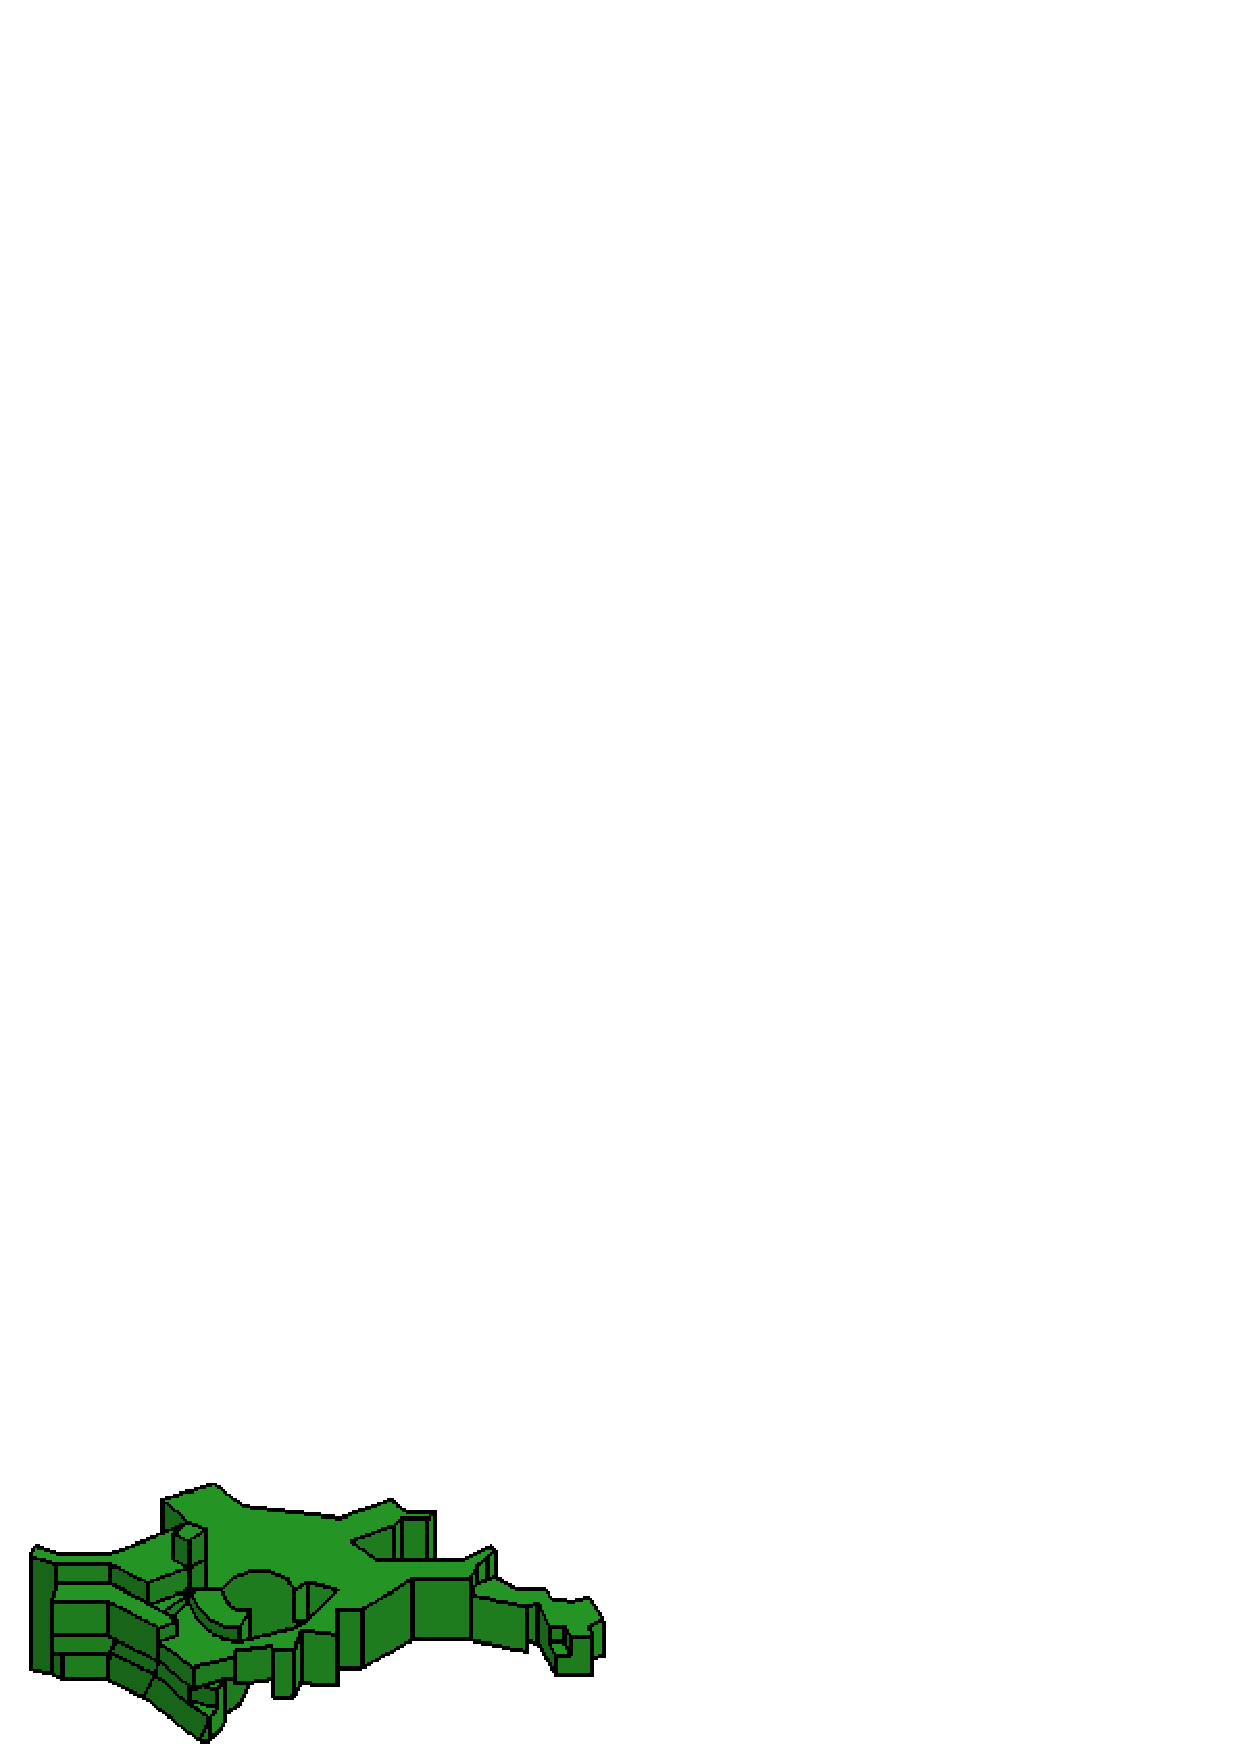
\includegraphics[width=4cm]{images/mpa_logo.pdf}

	\Large Max-Planck-Institut f\"ur Astrophysik\\


        \begin{table}[t]
	\begin{tabular}{c c c}
%       \begin{figure}[h]
        \includegraphics[width=1.0in,angle=90]{images/TUM.pdf}
%	\end{figure}
%	\vspace*{\stretch{1}}
	& &
%       \vspace*{\stretch{3}}
%       \begin{figure}[h]
	
\includegraphics[width=1.0in]{images/PH_CMYK.pdf}\\
%	\end{figure}
%	\vspace*{\stretch{1}}
        \Large Technische Universit\"at M\"unchen
	\vspace*{\stretch{1}}
	& &
	\Large Physik Department\\
%       \vspace*{\stretch{1}}
        \hspace*{0.1\linewidth}
        &
	\hspace*{0.2\linewidth}
        &
	\hspace*{0.2\linewidth}\\
        \end{tabular}
	\end{table}
  \end{center}
  \cleardoublepage
}

\setlength{\parskip}{2.0ex plus0.5ex minus0.5ex}
\setlength{\parindent}{0em}

% Alter some LaTeX defaults for better treatment of figures:
% See p.105 of "TeX Unbound" for suggested values.
% See pp. 199-200 of Lamport's "LaTeX" book for details.
%   General parameters, for ALL pages:
\renewcommand{\topfraction}{0.9}	% max fraction of floats at top
\renewcommand{\bottomfraction}{0.8}	% max fraction of floats at bottom
%   Parameters for TEXT pages (not float pages):
\setcounter{topnumber}{1}
\setcounter{bottomnumber}{2}
\setcounter{totalnumber}{4}     % 2 may work better
\setcounter{dbltopnumber}{2}    % for 2-column pages
\renewcommand{\dbltopfraction}{0.9}	% fit big float above 2-col. text
\renewcommand{\textfraction}{0.07}	% allow minimal text w. figs
%   Parameters for FLOAT pages (not text pages):
\renewcommand{\floatpagefraction}{0.7}	% require fuller float pages
% N.B.: floatpagefraction MUST be less than topfraction !!
\renewcommand{\dblfloatpagefraction}{0.7}	% require fuller float pages

% remember to use [htp] or [htpb] for placement

\makeatletter
\newcommand\footnoteref[1]{\protected@xdef\@thefnmark{\ref{#1}}\@footnotemark}
\makeatother

\newcommand{\grad}[0]{\mathbf{grad}\thinspace}
\renewcommand{\div}[0]{\text{div}\thinspace}
\newcommand{\curl}[0]{\mathbf{curl}\thinspace}
\renewcommand{\v}[0]{\mathbf}

\newcommand{\partt}[1]{\frac{\partial #1}{\partial t}}
\newcommand{\mean}[1]{\langle #1 \rangle}
\newcommand{\var}{\text{var}}


\newcommand{\beq}{\begin{equation}}
\newcommand{\eeq}{\end{equation}}
\newcommand{\beqn}{\begin{eqnarray}}
\newcommand{\eeqn}{\end{eqnarray}}
\renewcommand{\vec}{\mathbf}

\newcommand{\ud}{\ensuremath{\mathrm{d}}}
\newcommand{\kmpers}{\ensuremath{\mathrm{km\,s}^{-1}}}
\newcommand{\ms}{\ensuremath{\mathrm{ms}}}
\newcommand{\msun}{{\ensuremath{M_\odot}}}
\newcommand{\msf}{{\ensuremath{M_\mathrm{4}}}}
\newcommand{\scc}{{\ensuremath{\mu_{4}}}} %mass accretion criterion
\newcommand{\mfe}{{\ensuremath{M_\mathrm{Fe}}}}
\newcommand{\xsi}{{\ensuremath{\xi_{1.5}}}}
\newcommand{\XSI}{{\ensuremath{\xi_{2.5}}}}

\newcommand{\PNS}  [0]{proto-neutron star}
\newcommand{\KEP}  [0]{\textsc{Kepler}}
\newcommand{\PROM} [0]{\textsc{Prometheus}}
\newcommand{\PHOTB}[0]{\textsc{Prometheus-Hotb}}
\newcommand{\PVERT}[0]{\textsc{Prometheus-Vertex}}
\newcommand{\HOTB} [0]{\textsc{Hotb}}

\newcommand{\ccsn} [0]{core-collapse supernova}
\newcommand{\ccsne}[0]{core-collapse supernovae}
\newcommand{\Ccsn} [0]{Core-collapse supernova}
\newcommand{\Ccsne}[0]{Core-collapse supernovae}
\newcommand{\CCSNe}[0]{Core-Collapse Supernovae}

\newcommand{\EOSs}[0]{equation of states}
\newcommand{\EOS}[0]{equation of state}
\newcommand{\FBH}[0]{FBH}
\newcommand{\rhor}[0]{$\rho r^3$} 
\newcommand{\TODO}[0]{\colorbox{red}{\textcolor{white}{TODO}} }
\newcommand{\BLUE}[1]{\textcolor{blue}{#1}}
\newcommand{\RED} [1]{\textcolor{red}{#1}}



%%%%%%%%%%%%%%%%%%%%%%%%%%%%
%%  Beginn des Dokuments  %%
%%%%%%%%%%%%%%%%%%%%%%%%%%%%`?

\begin{document}
\thispagestyle{empty}
\begin{center}

\bgroup
\tabcolsep=10mm
\makebox[\linewidth]{
  \begin{tabular}{cc}
  \includegraphics[width=4cm]{front_page/tum} &
  \includegraphics[width=4cm]{front_page/mpa} \\[2mm]
  \large{Technische Universit\"at M\"unchen} & \large{Max-Planck-Institut f{\"u}r Astrophysik}
  \end{tabular}}
  \egroup

  \vspace*{1.8cm}

  \noindent

  \titletitlefont{\thesistitle}

  \vspace*{0.7cm}

  \noindent
  \titlenamefont{Haakon Andresen}

  \end{center}

  \vspace*{1cm}

  \noindent
  Vollst\"andiger Abdruck der von der Fakult\"at f\"ur Physik der Technischen
  Universit\"at M\"unchen zur Erlangung des akademischen Grades eines

  \begin{center}
  \titledoktorfont{Doktors der Naturwissenschaften (Dr. rer. nat.)}
  \end{center}

  \noindent
  genehmigten Dissertation.

  \vspace*{1cm}

  \begin{tabular}{lll}
  Vorsitzender: & & Univ.-Prof. Dr. \\
  Pr\"ufer der Dissertation: & 1. & Priv.-Doz.  \\
			     & 2. & Univ.-Prof.  \\
                             & 3. & Univ.-Prof. 
  \end{tabular}

\vspace*{1cm}
\noindent
   Die Dissertation wurde am xx.xx.2017 bei der Technischen Universit\"at M\"unchen
   eingereicht und durch die Fakult\"at f\"ur Physik am xx.xx.2017 angenommen.
  \selectlanguage{english}
 % \clearpage
 % \input{abstract.tex}

  \cleardoublepage
%  \pagenumbering{roman}

  \tableofcontents

  \newpage\null\thispagestyle{empty}\newpage

  \mainmatter
  \pagenumbering{arabic}
  \setcounter{page}{1}


%hier einzelne Kapitel einbinben
% \include{chapter/intro}

    % !! CHAPTERS GO HERE !!


%  \input{chapter/introduction.tex}

  
%%% Local Variables:
%%% mode: latex
%%% TeX-master: "../../doktorarbeit"
%%% End:

\chapter{Supernovae}
The history of supernovae starts, as most astrophysical objects, with observations of strong
electromagnetic events in the night sky. Supernovae are some of the most energetic events
known to astronomers and throughout history some have been clearly visible from earth and could be 
seen even during the day (see \cite{hamacher_14} and references therein). 
The Crab supernova was in 1054 described by Chinese astronomers \citep{ho_96,shen_96}. 
\begin{displayquote}
\textit{... it was visible by day, like Venus; pointed rays shot out
from it on all sides; the color was reddish-white. Altogether it
was visible for 23 days.}
\end{displayquote}
\section{Classifying supernovae}
In the modern era observations of supernovae continually improved. In 1941
German-American astronomer Rudolph Minkowski \citep{minkowski_41} found
that not all supernovae show hydrogen lines in their spectra and
he consequently divided supernovae into two types based on the
presence of hydrogen (Type II) or lack of hydrogen lines (Type I).
Later it was recognized that there were variations within these two classes
and a set of sub-classes, based on variation in the spectra and light curve. 
Type I supernovae were divided into type Ia, Ib and Ic,
where the nebular spectrum of types Ib and Ic was found to be similar to
those of type II supernovae. Two examples of the type II sub-classes are
types II-L and II-P. After reaching the maximum luminosity, the light curves of type II-P supernovae settles onto a
plateau and their luminosity reminds almost constant for several months. The luminosity of Type II-L, on the other hand, 
decline almost linearly. For a detailed reviwe of the classification system see \cite{cappellaro_01}.

The similarities between the nebular spectra of type II and type Ib/c supernovae already hints at a similar 
explosion mechanism. From a theoretical stand point one might say that a classification based on physical processes
powering the supernovae is more prudent. Already in 1960 \cite{hoyle_60} suggested that type II supernovae results from
the implosion of stellar cores and that type I is produced by igniting degenerate stellar material. Today it is understood that
that type Ia supernovae result from the thermonuclear explosions of white dwarfs, in other words the ignition of degenerate stellar material.
Furthermore, we now know that type II and type Ib/c supernovae are the result of the gravitational collapse, the implosion, of stellar cores.
The later category are known as core-collapse supernovae. The subject of this thesis is the gravitational waves generated during the 
collapse and subsequent explosion of a specific sub-type of core-collapse supernova, the ``Iron-core supernova'', and we therefor 
constrain our attention to this class of supernovae. The interested reader is refereed to \cite{janka_12} for a comprehensive description 
of the possible explosion mechanisms.

\section{Iron-core supernovae}
\subsection{Shell burning in massive stars}
\begin{wrapfigure}{r}{0.5\textwidth} \label{figSN:onion}
\begin{tikzpicture}[scale=0.8]
\definecolor{c1}{RGB}{141,211,199}
\definecolor{c2}{RGB}{255,255,179}
\definecolor{c3}{RGB}{190,186,218}
\definecolor{c4}{RGB}{251,128,114}
\definecolor{c5}{RGB}{128,177,211}
\definecolor{c6}{RGB}{253,180,98}
\definecolor{c7}{RGB}{179,222,105}
\fill[c7!80] (0,0) circle (5.2cm);
\fill[c6!80] (0,0) circle (4.5cm);
\fill[c5!80] (0,0) circle (3.8cm);
\fill[c4!80] (0,0) circle (3.1cm);
\fill[c3!80] (0,0) circle (2.4cm);
\fill[c2!80] (0,0) circle (1.7cm);
\fill[c1!80] (0,0) circle (1cm);
\node at (0,0.3) {\Large{Fe-Ni}};
\node at (0,-0.3) {\Large{core}};
\node at (0,1.3) {\Large{Si}};
\node at (0,2.) {\Large{O}};
\node at (0,2.7) {\Large{Ne}};
\node at (0,3.4) {\Large{C}};
\node at (0,4.1) {\Large{He}};
\node at (0,4.8) {\Large{H}};
\end{tikzpicture}
\caption{Schematic representation of the shell structure of a massive star right before
the onset of core-collapse. The stellar core consists of consecutive layers where heavier
and heavier elements are burned and a inner iron-nickel core.}
\end{wrapfigure}
When a massive star nears the end of its life it has depleted most of the hydrogen in the central core
and hydrogen burning ceases and the gravitational pull is no longer balanced by radiation pressure resulting
from nuclear fusion. The consequence is that the core starts to contract, the contraction is eventually halted when the pressure
and temperature in the core becomes large enough for helium burning to set in. The layer right outside of the helium burning core is still rich
in hydrogen and so hydrogen burning develops in a layer around the core. The burning of helium in the core stabilises the star, for a while.
However, the helium fuel eventually runs out and the process repeats itself, only this time the contraction continues until carbon ignites in the inner core. 

The process of burning heavier and heavier elements in the core continues up to silicon. The end product of silicon burning is iron-group elements and
since nuclear fusion of iron-group elements does not release any energy the cycle stops at silicon. The end result of this process is
an onion like shell structure consisting of consecutive layers burning heavier and heavier elements. In the centre of this onion is ever growing
core consisting of iron and nickel (hence forth refereed to as the ``iron-core''), it grows due to the ashes produced by the continued burning of silicon in the layer above. A depiction of this shell structure can be seen in \fig{figSN:onion}.
The star remains in this state for a while,
until the central iron-core has accumulated so much matter that its mass exceeds the Chandrasekhar mass and the inevitable gravitational collapse 
of the core begins.
% As John Connor, the star has no hopes of stopping judgement day, it can only hope to postpone it. 
% Gravitational collapse is, as the terminator puts it, inevitable.

\subsection{Iron-core collapse}
The collapse of the iron-core is triggerd and accelarated by two processes.
Firstly, rising temperatures increases the rate of photo-dissociation of iron-group 
nuclei. The nuclei is converted into free nucleons and alpha particles,
witch is a process that consumes thermal energy. Secondly, as the core density increases electron capture
on heavy nuclei becomes more frequent. Free electrons are capture by protons in the nuclei and an neutrons 
and anti-electron neutrinos are produced:
\begin{equation} \label{eqSN:ecapture}
p^{+} + e^{-} \rightarrow n - \bar{\nu}
\end{equation},
were $p^{+}$, $e^{-}$, $n$ and $\bar{\nu}$ represents a proton, an electron, 
a neutron and an anti-electron neutrino, respectively.
The neutrinos escape the core and in the process carry with them energy
and lepton number. With the loss of lepton numbers the mass the pressure from
degenerate electron decreases, effectively reducing the Chandrasekhar mass of the core. 

The deleptonisation of the iron-core eventually stops, at densities around $10^{12}$ g/cm$^3$ the
mean free path of the neutrinos become so short that the time they need to diffuse out of the
core is larger than the time-scale of the collapse. The iron-core, therefor, from this point on collapses in a 
adiabatic and homologous manner. The collapse continues until the central iron-core reaches nuclear densities, around $2.7 \times 10^{14} $g/cm$^3$,
at this point the repulsive forces between nuclei leads to a sudden stiffening of the equation of state (EoS) and the collapse of the
inner iron-core comes to an abrupt halt. 

However, due to its high inertia the inner core contracts beyond the equilibrium point of the
gravitational pull and its new found pressure source. This leads to a recoil and as the inner region of the iron-core expands outwards it crashes
into the infalling material above it. This event is the so called core bounce and it launches a sound wave into the outer iron-core, that 
steepens into a shock wave when it reaches the supersonically infalling layers of the outer core.

As the shock propagates outwards through the dens stellar material it loses about 
$10^{51}$ erg of energy per 0.1 \msun of iron-core material that falls through the shock front, 
due to the dissociation of heavy nuclei, falling through the shock, into free nucleons.
Eventually the density ahead of the shock drops below $\sim \, 10^{11}$ g/cm$^3$ and
the neutrinos behind the shock can suddenly escape. This leads to a burst of neutrino 
emission and a significant loss of energy for the shock. After a few milliseconds the
shock has lost so much energy that it stalls at a radius between 100 and 200 km
and turns into an accretion shock. In order to s




  
  \cleardoublepage
  \thispagestyle{empty}
  
%%% Local Variables:
%%% mode: latex
%%% TeX-master: "../../doktorarbeit"
%%% End:

\chapter{Theory}


\section{General relativity}
The total gravitational action is given by the sum of the 
Einstein action, $S_E$, and the matter action, $S_M$.
\begin{equation}
S_E = \frac{c^3}{16 \pi G} \int \mathrm{d}^4 x \sqrt{-g} R
\end{equation}


\section{Linearised theory}
One of the most straight forward ways to understand 
GWs is to expand the Einstein equations around the 
flat Minkowski space. Mathematically this means that we write the
metric tensor $\munu{g}$ as
\begin{equation} \label{eqT:metric}
\munu{g} = \munu{\eta} + \munu{h},
\end{equation}
where $\munu{\eta}$ is the Minkowski metric tensor and $\munu{h}$
is some small perturbation satisfying the condition
\begin{equation} \label{eqT:hsmall}
|\munu{h}|  \ll 1.
\end{equation}
The condition given by Eq.~\ref{eqT:hsmall} will not hold in a arbitrary 
reference frame. Therefor, by imposing the smallness condition on $\munu{h}$
we implicitly chose a frame where the numerical value of the components of $\munu{h}$ is much smaller than one,
in the region of space which we are interested in. In linearised theory we use the Minkowski metric tensor
to lower and raise indices. 

The field equations of general relativity can
be written in terms of the Ricci tensor ($\munu{R}$), the Ricci scalar ($R$), the metric tensor,
and the energy-momentum tensor ($\munu{T}$) as follows
\begin{equation} \label{eqT:einstein}
\munu{R} - \frac{1}{2} \munu{g} R = \frac{8 \pi G}{c^4 } \munu{T}. 
\end{equation}
Before we combine Eq.~\ref{eqT:metric} and Eq.~\ref{eqT:einstein} we introduce the simplifying notation
\begin{equation} \label{eqT:h}
h = \munut{\eta}\munu{h},
\end{equation}
and
\begin{equation} \label{eqT:hbar}
\munu{\bar{h}} = \munu{h} - \frac{1}{2}\munu{\eta}h.
\end{equation}
By inserting our expression for the metric tensor (Eq.~\ref{eqT:metric}) into Eq.~\ref{eqT:einstein}
and expand to linear order in $\munu{h}$ we find the linearised version of the Einstein equations
\begin{equation} \label{eqT:einlin}
\partial_{\gamma} \partial^{\gamma} \munu{\bar{h}} + \munu{\eta} \partial^{\rho} \partial^{sigma} \bar{h}_{\rho \sigma}
- \partial^{\rho}\partial_{\nu}\bar{h}_{\mu \sigma} -  \partial^{\rho}\partial_{\mu}\bar{h}_{\nu \sigma}
= \frac{8 \pi G}{c^4 } \munu{T}.
\end{equation}
We can simplify Eq.~\ref{eqT:einlin} by using the gauge freedom of our linearised theory to chose the Lorentz gauge,
\begin{equation} \label{eqT:lor}
\partial^{nu} \munu{\bar{h}} = 0.
\end{equation}
Under this gauge condition Eq.~\ref{eqT:einlin} reduces to a wave equation 
\begin{equation} \label{eqT:wave}
\partial_{\gamma} \partial^{\gamma} \munu{\bar{h}} = \frac{8 \pi G}{c^4 } \munu{T},
\end{equation}
since every term, except the first one, on the left hand side vanishes. 

Eq.~\ref{eqT:wave} further simplifies when we are outside of the sources generating
GWs, in vacuum the energy-momentum tensor vanishes and we get  
\begin{equation} \label{eqT:wavevacuum}
\partial_{\gamma} \partial^{\gamma} \munu{\bar{h}} = 0,
\end{equation}
which can be rewritten as
\begin{equation} \label{eqT:wavevacumm2}
\frac{1}{c^2} \partial_t^2 \munu{\bar{h}} = [ \partial_1^x  + \partial_y^2 + \partial_z^2] \munu{\bar{h}}.
\end{equation}
It is clear from the latter form that GWs propagate through spacetime at the speed of light in a wave-like fashion.

\section{The transverse-traceless gauge}
Even though we introduced the Lorentz gauge earlier, we have not completely removed all superfluous degrees of freedom 
in the linearised field equations. In vacuum, where the energy-momentum tensor vanishes and Eq.~\ref{eqT:wavevacumm} holds, it is possible
to simplify the expression for $\munu{h}$. The transverse-traceless gauge (we will denote the transverse-traceless gauge
with TT and quantities with a TT are understood to be in the TT-gauge) imposed the following conditions
\begin{equation} \label{eqT:ttg}
h^{0 \mu} = 0, \qquad h^{i}_{i} = 0, \qquad \text{and} \qquad \partial^j h_{ij} = 0.
\end{equation}
The solutions to Eq.~\ref{eqT:wavevacumm} are plane wave solutions and in the TT-gauge the 
solution for a plane wave propagating along the z-axis is given by
\begin{equation} \label{eqT:hzdir}
h_{ij}^{TT}=
  \begin{pmatrix}
    h_{+} & h_{\times} & 0  \\
    h_{\times} & -h_{+} & 0 \\
    0 & 0 & 0
  \end{pmatrix}_{ij}
  cos[\omega(t - z/c)].
\end{equation}
Here we $t$ denotes time, $\omega$ the angular frequency of the wave,
$h_+$ denotes the wave strain of the plus-polarised mode and $h_{\times}$ is the strain amplitude of the cross-polarised mode.
To prove that we can impose the conditions of Eq.~\ref{eqT:ttg} we start by
realising that the Lorentz gauge does not completely constrain the theory by considering the 
coordinate transformation 
\begin{equation} \label{eqT:ct}
x^{\mu} \rightarrow x^{'\mu} = x^{\mu} + \epsilon^{\mu},
\end{equation}
where $\epsilon^{\mu}$ satisfy $\partial_{\gamma} \partial^{\gamma} \epsilon_{\mu} = 0$ 
and $|\partial_{\nu} \epsilon_{\mu}|$ is at the most on the order of $|\munu{h}|$.
Under an arbitrary coordinate transformation $x^{\mu} \rightarrow x^{'\mu}(x)$ the second rank tensor $\munu{h}$ transforms as
\begin{equation} \label{eqT:t2c}
\munu{h} \rightarrow \munu{h'} = \frac{\partial x^{\gamma}}{\partial x^{'\mu}} \frac{\partial x^{\sigma}}{\partial x^{'\nu}} h_{\gamma \sigma}.
\end{equation}
Evaluating Eq.~\ref{eqT:t2c} for the coordinate transformation given by Eq.~\ref{eqT:ct} gives
\begin{equation} \label{eqT:htrans}
\munu{h} \rightarrow \munu{h'} = \munu{h} - (\partial_{\mu} \epsilon_{\nu} + \partial_{\nu} \epsilon_{\mu}). 
\end{equation}
By combining Eq.~\ref{eqT:htrans} and Eq.~\ref{eqT:hbar} we find that under Eq.~\ref{eqT:ct} $\munu{\bar{h}}$ transforms as follows
\begin{equation} \label{eqT:hbartrans}
\munu{\bar{h}} \rightarrow \munu{\bar{h}'} =  \munu{{h}} - (\partial_{\mu} \epsilon_{\nu} + \partial_{\nu} \epsilon_{\mu} - \munu{\eta}\partial_{\gamma} \epsilon^{\gamma}). 
\end{equation}
By applying  $\partial_{\mu}$ to Eq.~\ref{eqT:ct} we find
\begin{equation} \label{eqT:dert}
\partial_{\mu} x^{'\mu} = \partial_{\mu} x^{\mu} + \partial_{\mu} \epsilon^{\mu},
\end{equation}
since $|\partial_{\mu} \epsilon^{\mu}| \ll 1$ Eq.~\ref{eqT:dert} implies that
\begin{equation}
\partial_{\mu} x^{'\mu} = \frac{\partial x^{'\mu} }{\partial x^{\mu}} = 1.
\end{equation}
This means that under the transformation given by Eq.~\ref{eqT:ct} the derivatives
transforms as follows
\begin{equation} \label{eqT:dert2}
\partial_{\mu} \rightarrow \partial_{\mu}^{'} = \partial_{\mu}.
\end{equation}
We can now calculate how Eq.~\ref{eqT:lor} transform under Eq.~\ref{eqT:ct}
\begin{align} \label{eqT:lort}
\partial^{\nu} \munu{\bar{h}} & \rightarrow (\partial^{\nu} \munu{\bar{h}})^{'} \\ \nonumber
&= \partial^{\nu} \left [ \munu{\bar{h}} - (\partial_{\mu} \epsilon_{\nu} + \partial_{\nu} \epsilon_{\mu} - \munu{\eta}\partial_{\gamma} \epsilon^{\gamma}) \right ] \\
&= \partial^{\nu} \munu{\bar{h}} - \partial^{\gamma} \partial_{\gamma} \epsilon_{\mu} = 0. \nonumber
\end{align}
We can now directly see that the transformation does not break the Lorentz gauge condition.

Instead of thinking about how $\munu{\bar{h}}$ transform under Eq.~\ref{eqT:ct}
we can instead think about it like this: Eq.~\ref{eqT:hbartrans} tells us that
that from four independent functions $\epsilon_{mu}$ we can construct the functions 
\begin{equation}
\munu{\epsilon} \equiv \partial_{\mu} \epsilon_{\nu} + \partial_{\nu} \epsilon_{\mu} - \munu{\eta}\partial_{\gamma} \epsilon^{\gamma}
\end{equation}
and are free to subtract this functions from $\munu{\bar{h}}$ without breaking the gauge condition set by Eq.~\ref{eqT:lor}.
With this freedom we can now choose the four functions such that they impose four simplifying conditions on  $\munu{h}$.
In the TT-gauge the four functions are chosen in such a that the trace of $\munu{\bar{h}}$ is zero and
so that $h^{0i} = 0$. Note that if the trace of $\munu{\bar{h}}$ vanishes then $\munu{\bar{h}} = \munu{h}$.
These four conditions, together with the Lorentz gauge, is what defines the TT-gauge and results in the
conditions set by Eq.~\ref{eqT:ttg}.

\section{Generation of gravitational waves}
We turn now to the to the generation of gravitational waves, in the linearised theory framework,
we start by writing down of Eq.~\ref{eqT:einlin} for a generic source under the assumption 
that the gravitational field generated by the source is weak enough to justify the expantion
around flat spacetime. 

As for any wave equation, the solution of \eq{eqT:einstein} can be found by integrating over the source
\begin{equation} \label{eqT:sol}
\munu{\bar{h}}(t,\matbf{x}) = \frac{4G}{c^4} \int \mathrm{d}^3 x' \frac{\munu{T}(t-|\mathbf{x}-\mathbf{x'}|/c}{|\mathbf{x}-\mathbf{x'}|}.
\end{equation}
Far way from the source at a distance $D$, if the velocities ($v$) within the source is small compared to the speed of light, \eq{eqT:sol} reduces to the Einsteins famous quadrupole expression. In the TT-gauge the quadrupole expression can be written as follows  
\begin{equation} \label{eqT:equad}
\munu{h}(t,\matbf{x}) = \frac{1}{D} \frac{4G}{c^4} \left [P_{im} P_{jn} - \frac{1}{2} P_{ij} P_{mn} \right ] \ddot{Q}_{ij} (t -d/c),
\end{equation}
where $Q_{ij}$ is the the mass quadrupole moment that to leading order in $v/c$ is given by
\begin{equation} \label{eqT:quad}
Q_{ij} = \int \mathrm{d}^3 x \rho(t,\matbf{x})\left [x_{ij} - \frac{1}{3} \delta^{ij} x_l x_l \right ].
\end{equation}
$P_{ij} = \delta_{ij} -n_i n_j$ is the projection operator onto the plane transverse to the direction the wave is propagating in,
$\hat{n}_i = x_i / \sqrt{x_j _x^j}$. To find the equation describing $h_{+}$ and $h_{\times}$ for a wave propagating in the general direction
$\hat{n}$ we first consider a wave propagating along the z-axis in a coordinate system with axes $(x,y,z)$. 
If $\hat{n} = \hat{z}$ then $P_{ij}$ becomes and we find that 
\begin{equation} \label{eqT:pjz}
P_{im} P_{jn} - \frac{1}{2} P_{ij} P_{mn} \right ] \ddot{Q}_{ij} = 
  \begin{pmatrix}
    (\ddot{Q}_{11}-\ddot{Q}_{22})/2 & \ddot{Q}_{12} & 0  \\
    \ddot{Q}_{21} & (\ddot{Q}_{22} - \ddot{Q}_{11})/2 & 0 \\
    0 & 0 & 0
  \end{pmatrix}_{ij}.
\end{equation}
By comparing \eq{eqT:hzdir} and \eq{eqT:pjz} we see that
\begin{align} \label{eqT:zhchx}
h_{+}^{TT} &= \frac{G}{c^4 D} (\ddot{Q}_{11}-\ddot{Q}_{22}) \\ \nonumber
h_{\times}^{TT} &= frac{2G}{c^4 D} \ddot{Q}_{12}.
\end{align}
Now consider a wave propegating along the $\hat{n} = (\sin{\theta} \sin{\phi}, \sin{\theta} \cos{\phi},\cos{\theta})$.
We can view this as a wave propagating along the z'-axis of a coordinate system, with axes $(x',y',z')$, that has been constructed  
by rotating the original system about the z-axis by an angle $\phi$ and then about the x-axis by an angle $\theta$. $h_{+}$ and $h_{\times}$.
The rotation matrix R of the two consecutive rotations is
\begin{equation} \label{eqT:pjz}
R = 
  \begin{pmatrix}
    \cos{\phi} & \sin{\phi} & 0  \\
    -\sin{\phi} & \cos{\phi} & 0 \\
    0 & 0 & 0
  \end{pmatrix}
  \begin{pmatrix}
    0 & 0 & 0  \\
    0& \cos{\theta} & \sin{\theta} \\
    0 & \cos{\theta} & \cos{\theta}
  \end{pmatrix}
\end{equation}

Since the wave propegates along the z'-direction we can use the result from before (\eq{eqT:zhchx})
\begin{align} \label{eqT:zhchxp}
h_{+}^{TT} &= \frac{G}{c^4 D} (\ddot{Q}_{11}'-\ddot{Q}_{22}') \\ \nonumber
h_{\times}^{TT} &= frac{2G}{c^4 D} \ddot{Q}_{12}'.
\end{align}
A second rank tensor, like the quadrupole tensor, transforms under as follows

\begin{eqnarray}
\label{eq:qtp}
\ddot{Q}_{\theta \phi} =&  \left (\ddot{Q}_{22} - \ddot{Q}_{11} \right ) \cos{\theta}\sin{\phi}\cos{\phi} \nonumber \\
&+ \ddot{Q}_{12} \cos{\theta} \left (\cos^2 \phi - \sin^2 \phi \right ) \nonumber \\ 
&+ \ddot{Q}_{13} \sin \theta \sin \phi - \ddot{Q}_{23} \sin \theta \cos\phi,
\end{eqnarray}
\begin{eqnarray}
\ddot{Q}_{\phi \phi} &= \ddot{Q}_{11} \sin^2 \phi + \ddot{Q}_{22} \cos^2 \phi - 2 \ddot{Q}_{12} \sin{\phi}\cos{\phi}
\end{eqnarray}
and
\begin{eqnarray}
\ddot{Q}_{\theta \theta} &= \left ( \ddot{Q}_{11} \cos^2 \phi + \ddot{Q}_{22} \sin^2 \phi +  2 \ddot{Q}_{12} \sin{\phi} \cos{\phi} \right) \cos^2 \theta \nonumber \\
&+ \ddot{Q}_{33} \sin^2 \theta - 2 \left (\ddot{Q}_{13} \cos{\phi} + \ddot{Q}_{23} \sin{\phi} \right ) \sin{\theta} \cos{\theta}. 
\end{eqnarray}


In the transverse traceless (TT) gauge and the far-field limit the metric perturbation, $\mathbf{h^\mathrm{TT}}$, 
can be expressed in terms of the amplitudes of the two independent polarisation modes in the following way,
\begin{equation}
\mathbf{h}^\mathrm{TT}(\mathbf{X},t) = \frac{1}{D}   \left [ A_{+} \mathbf{e}_{+} + A_{\times} \mathbf{e}_{\times} \right ].
\end{equation}
Here, $D$ denotes the distance between the source and the observer, $A_+$ denotes the wave amplitude of the plus-polarised mode, $A_\times$ is the wave amplitude of the cross-polarised mode and
$\mathbf{e}_{\times}$ and $\mathbf{e}_{+}$ denote the unit polarisation tensors. The unit polarisation tensors are given by
\begin{equation}
\mathbf{e}_{+}  = \mathbf{e}_{\theta} \otimes \mathbf{e}_{\theta} - \mathbf{e}_{\phi} \otimes \mathbf{e}_{\phi},
\end{equation}
\begin{equation}
\mathbf{e_{\times}} = \mathbf{e}_{\theta} \otimes \mathbf{e}_{\phi} + \mathbf{e}_{\phi} \otimes \mathbf{e}_{\theta},
\end{equation}
where $\mathbf{e}_{\theta}$ and $\mathbf{e}_{\phi}$ are the unit vectors in the $\theta$ and $\phi$
direction of a spherical coordinate system and $\otimes$ denotes the tensor product.
Using the quadrupole approximation in the slow-motion limit, the amplitudes $A_{\times}$ and $A_{+}$ can be computed from the second time derivative 
of the symmetric trace-free (STF) part of the mass quadrupole tensor $Q$~\citep{oohara_97},
\begin{equation}
\label{eq:aplus}
A_{+} = \ddot{Q}_{\theta \theta} - \ddot{Q}_{\phi \phi},
\end{equation}
\begin{equation}
\label{eq:ax}
A_{\times} =2 \ddot{Q}_{\theta \phi}.
\end{equation}
The components of $Q$ in the orthonormal basis associated with
spherical polar coordinates used in this formula can be obtained from
the Cartesian components $\ddot{Q}_{ij}$ of $\ddot{Q}$ \citep{oohara_97,nakamura_87}.  Using the
continuity and momentum equations to eliminate time derivatives
\citep{oohara_97,finn_89,blanchet_90}, the Cartesian components can be obtained as:
\begin{equation} \label{eq:STFQ}
\ddot{Q}_{ij} =\mathrm{STF} \left [2 \frac{G}{c^4} \int \ud^3 x \, \rho \left ( v_i v_j - x_i \partial_j \Phi \right ) \right].
\end{equation}
Here, $G$ is Newton's gravitational constant, $c$ is the speed of
light, and $v_i$ and $x_i$ are the Cartesian velocity components and
coordinates ($i = 1,2,3$), respectively. The gravitational potential
$\Phi$ is the gravitational potential used in the simulations (with post-Newtonian
corrections taken into account). $\mathrm{STF}$ denotes the projection operator
onto the symmetric trace-free part.
The advantage of this form is that
the second-order time derivatives are transformed into first-order
spatial derivatives, thus circumventing problems associated with the
numerical evaluation of second-order time derivatives. 
Using standard
coordinate transformations between Cartesian and spherical
coordinates, we obtain \citep{oohara_97,nakamura_87} the components 
$\ddot{Q}_{\theta \theta}$, $\ddot{Q}_{\phi \phi}$, and
$\ddot{Q}_{\theta \phi}$ needed in Eq.~(\ref{eq:aplus}) and (\ref{eq:ax}),
\begin{eqnarray}
\label{eq:qtp}
\ddot{Q}_{\theta \phi} =&  \left (\ddot{Q}_{22} - \ddot{Q}_{11} \right ) \cos{\theta}\sin{\phi}\cos{\phi} \nonumber \\
&+ \ddot{Q}_{12} \cos{\theta} \left (\cos^2 \phi - \sin^2 \phi \right ) \nonumber \\ 
&+ \ddot{Q}_{13} \sin \theta \sin \phi - \ddot{Q}_{23} \sin \theta \cos\phi,
\end{eqnarray}
\begin{eqnarray}
\ddot{Q}_{\phi \phi} &= \ddot{Q}_{11} \sin^2 \phi + \ddot{Q}_{22} \cos^2 \phi - 2 \ddot{Q}_{12} \sin{\phi}\cos{\phi}
\end{eqnarray}
and
\begin{eqnarray}
\ddot{Q}_{\theta \theta} &= \left ( \ddot{Q}_{11} \cos^2 \phi + \ddot{Q}_{22} \sin^2 \phi +  2 \ddot{Q}_{12} \sin{\phi} \cos{\phi} \right) \cos^2 \theta \nonumber \\
&+ \ddot{Q}_{33} \sin^2 \theta - 2 \left (\ddot{Q}_{13} \cos{\phi} + \ddot{Q}_{23} \sin{\phi} \right ) \sin{\theta} \cos{\theta}. 
\end{eqnarray}

In axisymmetry the only independent component of $\mathbf{h}^\mathrm{TT}$ is 
\begin{equation}
\mathbf{h}^\mathrm{TT}_{\theta \theta} = \frac{1}{8}\sqrt{\frac{15}{\pi}} \sin^2{\theta} \frac{A_{20}^\mathrm{E2}}{D},
\end{equation}
where $D$ is the distance to the source, $\theta$ is the inclination angle of the observer with respect to the
axis of symmetry, and $A_{20}^\mathrm{E2}$ represents the only non-zero quadrupole amplitude.
In spherical coordinates $A_{20}^\mathrm{E2}$ can be expressed as follows
\begin{eqnarray} \label{eq:2dquad}
A_{20}^\mathrm{E2} (t) =  \frac{G}{c^4} \frac{16 \pi^{3/2}}{\sqrt{15}} \int_{-1}^{1}\int^{\infty}_0 \rho \left [ v_r^2(3 z^2 - 1)+ \right. \nonumber \\
v_{\theta}^2(2-3 z^2) - v_{\phi}^2 - 6 v_r v_{\theta} z\sqrt{1-z^2} + \nonumber \\
r \partial_r \Phi (3 z^2 - 1) +\left. 3 \partial_{\theta}z\sqrt{1-z^2} \Phi \right ]r^2 dr \, dz.
\end{eqnarray}
Here, $v_i$ and $\partial_i$ ($i = r, \theta, \phi$) represent the velocity components and derivatives, respectively, along
the basis vectors of the spherical coordinate system, and $z \equiv \cos \theta$.
For details we refer the reader to \cite{mueller_97}.


  \cleardoublepage
  \thispagestyle{empty}

  
%%% Local Variables:
%%% mode: latex
%%% TeX-master: "../../doktorarbeit"
%%% End:
\chapter{Numerical simulations of core-collapse supernovae}
The GW signals presented in this thesis is based on 
supernova simulations that were performed with the code \textsc{Prometheus-Vertex}.
The simulations were carried out by members of the Garching-group 
(\cite{hanke_phd,melson_phd,suma_models}).
In this chapter we described the code that was used, we will
describe the details of individual models in later chapters. 
\textsc{Prometheus-Vertex} solves the combined problem of hydrodynamics and neutrino radiation transport.
The code has been specifically developed for the core-collapse problem,
the first version was developed in 2002 by \cite{rampp_02} 

\section{\textsc{Prometheus}}
The hydrodynamics of the stellar collapse is solved with a version of the
well-established \textsc{Prometheus} code \citep{mueller_91,fryxell_91}. It solves the non-relativistic 
equations of hydrodynamics for the inviscid flow of an ideal fluid in spherical coordinates $(r,\theta,\phi)$.
\subsection{Hydrodynamics}
In spherical coordinates the Euler equations of hydrodynamics are 
\begin{alignat}{1}
&\partial_t \rho + \frac{1}{r^2} \partial_r (r^2 \rho v_r) + \frac{1}{r \sin{\theta}} \bigg[ \partial_{\theta} (\rho \sin{\theta} v_{\theta}) + \partial_{\phi} (\rho v_{\phi}) \bigg] = 0, \label{eqN:cont} \\
\stepcounter{equation}
&\partial_t (\rho v_r) + \frac{1}{r \sin{\theta}} \bigg[ \partial_{\theta} (\rho \sin{\theta} v_{\theta} v_r)
+\partial_{\phi} (\rho v_{\phi} v_r) \bigg]  + \nonumber \\ 
&\frac{1}{r^2} \partial_r (r^2 \rho v_r^2)  - \rho \frac{v_{\theta}^2 + v_{\phi}^2}{r} + \partial_r p 
= - \rho \partial_r \Phi + Q_{M_r}, \tag{\theequation{}a} \\
%
&\partial_t (\rho v_{\theta}) + \frac{1}{r^2} \partial_r (r^2 \rho v_r v_{\theta}) + \frac{1}{r \sin{\theta}}\bigg[ \partial_{\theta} (\rho \sin{\theta} v_{\theta}^2) +
\partial_{\phi} (\rho v_{\phi} v_{\theta}) \bigg] \nonumber \\
&+\rho \frac{v_{\theta}v_r - v_{\phi}^2/\tan{\theta}}{r} + \frac{1}{r}\partial_{\theta} p = - \frac{\rho}{r} \partial_{\theta} \Phi + Q_{M_{\theta}}, \tag{\theequation{}b} \\
%
&\partial_t (\rho v_{\phi})  
+\frac{1}{r \sin{\theta}} \bigg[ \partial_{\theta} (\rho \sin{\theta} v_{\theta} v_{\phi}) +
\partial_{\phi} (\rho v_{\phi}^2)  + \partial_{\phi} p  \bigg] \nonumber \\
&+ \frac{1}{r^2} \partial_r (r^2 \rho v_r v_{\phi}) +
\rho \frac{v_{\theta}v_{\phi}/\tan{\theta} + v_{\phi}v_r}{r}
 = -\frac{1}{r \sin{\theta}} \partial_{\phi} \Phi + Q_{M_{\phi}}, \tag{\theequation{}c} \\
%
\stepcounter{equation}
&\partial_t e + \frac{1}{r^2} \partial_r (r^2 v_r (e + p))
+\frac{1}{r \sin{\theta}} \bigg[ \partial_{\theta} ( \sin{\theta} v_{\theta} (e + p))  +
\partial_{\phi} (v_{\phi} (e + p)) \bigg] \nonumber \\
&= -\rho v_r \partial_r \Phi - \rho\frac{v_{\theta}}{r}\partial_{\theta}\Phi - \frac{v_{\phi}}{r \sin{\theta}} \partial_{\phi} \Phi
 + Q_E + v_r Q_{M_r} + v_{\theta} Q_{M_{\theta}} + v_{\phi} Q_{M_{\phi}}.
\end{alignat}
Here $p$ is pressure, $\rho$ is density, $e$ is the specific total energy,  $\Phi$ is the gravitational potential and
$v_r$, $v_{\theta}$, and $v_{\phi}$ are the velocity components in the spherical
coordinate basis. The source terms $Q_{M_{r}}$, $Q_{M_{\theta}}$, and $Q_{M_{\phi}}$ represent
momentum transfer by neutrinos, in the radial, polar, and azimuthal direction, respectively.
Energy transport by neutrinos is represented by the source term $Q_{M_{E}}$. These source terms are calculated
by the neutrino-transport module \textsc{Vertex}, which we will come back to them later in the chapter.
The above equations have to be closed by an EoS, which generally will depend on 
density, internal energy, and the chemical composition of the stellar matter.
This means that one has to track of two additional quantities, the mass fractions
of different nuclear species, denoted by $X_i$, and the electron fraction $Y_e$. We, therefore,
have to solve two additional conservation equations:
\begin{alignat}{1}
\partial_t (\rho X_i) + \frac{1}{r^2} \partial_r (r^2 \rho v_r X_i) + \frac{1}{r \sin{\theta}} \bigg[ \partial_{\theta} (\rho \sin{\theta} v_{\theta} X_i) + \partial_{\phi} (\rho v_{\phi} X_i) \bigg] &= \varsigma_i, \label{eqN:contxi} \\
\partial_t (\rho Y_e) + \frac{1}{r^2} \partial_r (r^2 \rho v_r Y_e) + \frac{1}{r \sin{\theta}} \bigg[ \partial_{\theta} (\rho \sin{\theta} v_{\theta} Y_e) + \partial_{\phi} (\rho v_{\phi} Y_e) \bigg] &= Q_{Y_e}. \label{eqN:contye}
\end{alignat}
The two terms $\varsigma_i$ and $Q_{Y_e}$ represents the change of composition of species $i$ due nuclear reactions
and the change in electron fraction caused by emission and absorption of electron and anti-electron neutrinos,
respectively. If the fluid reaches nuclear statistical equilibrium (NSE), then the chemical 
composition is fully determined by the equation of state, through the electron fraction, density, and
temperature.

\textsc{Prometheus} solves the system of equations described in the paragraph above
by means of a dimensionally-split implementation of the piecewise parabolic method of \cite{colella_84}.
The scheme is time-explicit and it is accurate to third-order in space and second-order in time.
The Riemann solver exactly solves 1D Riemann problems in so-called sweeps
that have been obtained from the full 3D equations by Strange-splitting \citep{strang_68}.
When strong shocks are encountered the solver switches to the ``HLLE'' solver \citep{einfeldt_88}.
This is done in order to avoid the so-called ``even-odd decoupling'', which occurs
when the shocks are aligned with one of the axes of the simulation grid \citep{quirk_94,kifonidis_03},
which creates artificial oscillations. \textsc{Prometheus} employs the 
consistent multi-fluid advection method of \cite{plewa_99} to ensure that the advection all the nuclear species
is calculated accurately.

\subsection{Equation of state}
The models that this work is based on uses two different prescriptions
for the EoS. A ``high-density'' EoS is used for the inner
hot region of the core, while a ``low-density'' EoS is used for the low-density regions of the simulation volume. The two are separated by a density threshold,
after core bounce this threshold is set to $\rho_T = 10^{11}$ g/cm$^3$.
In the high-density regime the tabular EoS of 
\cite{lattimer_91} with a nuclear incompressibility of 220 MeV is used. 
Below the threshold, in the low-density regime, an EoS that describes the nuclei as
classical Boltzmann gases. Electrons and positrons are described as Fermi gases with arbitrary degeneracy levels. The EoS also include the effect of photons \citep{janka_99}.

\subsection{Self gravity - the effective potential}
Self-gravity is treated using the monopole                      
approximation and the effects of general relativity are accounted for                                               
in an approximate fashion by means of a pseudo-relativistic                                                          
effective potential (case~A of \cite{marek_06}). 
The effective potential includes general relativistic effects and
takes the properties of the medium into account, such as the pressure and energy
of the fluid elements. In the case of a monopole potential, the terms involving
non-radial derivatives of the potential in the Euler equations vanish.

\section{\textsc{Vertex}}
The \textsc{Vertex} code calculates the source terms on the right-hand side of the
Euler equations by treating the neutrinos as a radiation field. 
The problem we need to solve is to find the phase-space distribution function $f(\mathbf{r},\mathbf{q},t)$ of the neutrinos.
Essentially we want to find the number of neutrinos momentum $\mathbf{q}$ at position $\mathbf{r}$, in other
words the number of particles in the phase-space volume $\mathrm{d} \mathbf{q} \mathrm{d} \mathbf{r}$.

It is common to work in terms of the specific intensity $\mathfrak{I}(\mathbf{r},\hat{n},\xi,t)$,
which is defined such that the amount of energy $d\xi$ transported in the energy interval
$(\xi,\xi+\mathrm{d}\xi)$, by neutrinos propagating into 
the solid angel $\mathrm{d}\Omega$ in the direction $\hat{n}$,
through a surface with area $\mathrm{d}A$, with normal vector $\hat{A} = \mathbf{r}/|\mathbf{r}|$, 
during the time interval $\mathrm{d}t$ is
\begin{equation} \label{eqN:intns}
d \xi = \mathfrak{I}(\mathbf{r},\hat{n},\xi,t) \, \hat{n} \cdot \hat{A}
\, \mathrm{d}\xi \, \mathrm{d}A \, \mathrm{d}\Omega \, \mathrm{d}t.
\end{equation}
The neutrino distribution function and the specific neutrino intensity is related as follows
\begin{equation}
\mathfrak{I}(\mathbf{r},\hat{n},\xi,t) = \frac{\xi^3}{h^3 c^2} f(\mathbf{r},\hat{n},\xi,t).
\end{equation}
The evolution of the specific neutrino intensity is calculated by solving the Boltzmann equation
\begin{equation} \label{eqN:boltz}
\frac{1}{c} \partial_t \mathfrak{I} + \hat{n}_i \partial_i \mathfrak{I} = \mathfrak{C} [\mathfrak{I}].
\end{equation}
The right hand side of \eq{eqN:boltz} is a source term that describes scattering, emission and absorption
of neutrinos (the so-called collision integral). $\mathfrak{C} [\mathfrak{I}]$ will in general depend on integrals of the specific neutrino intensity, witch makes the problem difficult to solve numerically. 
A common strategy is to expand the specific neutrino intensity into angular moments
\begin{alignat}{2}
\mathfrak{L}(\mathbf{r},\xi,t) &\equiv  \frac{1}{4\pi} \int \mathfrak{I} \, \mathrm{d} \Omega &&\qquad (\nth{0}-order), \\ 
\mathfrak{H}_i(\mathbf{r},\xi,t) &\equiv  \frac{1}{4\pi} \int \mathfrak{I} \, \hat{n}_i \, \mathrm{d} \Omega &&\qquad (\nth{1}-order), \\
\mathfrak{K}_{ij}(\mathbf{r},\xi,t) &\equiv  \frac{1}{4\pi} \int \mathfrak{I} \, \hat{n}_i \, \hat{n}_j \, \mathrm{d} \Omega &&\qquad (\nth{2}-\text{order}), \\
& \ \ \vdots && \nonumber
\end{alignat}
and then solve the equations that arises when inserting these moments into \eq{eqN:boltz}
\begin{align}
\frac{1}{c} \partial_t \mathfrak{L} +  \partial_i \mathfrak{H}_i &= \frac{1}{4\pi} \int \mathfrak{C} [\mathfrak{I}] \mathrm{d} \Omega, \\
\frac{1}{c} \partial_t \mathfrak{H}_i + \partial_i \mathfrak{K}_{ij} &= \frac{1}{4\pi} \int \mathfrak{C} [\mathfrak{I}] \hat{n}_i \mathrm{d} \Omega. \\
& \ \ \vdots \nonumber
\end{align}
We see from these equations that the evolution of the $k^{\text{th}}$-order moment depends on $(k+1)^{\text{th}}$-order moment.

The version of \textsc{Vertex} that is implemented into \textsc{Prometheus-Vertex} uses
the so-called``ray-by-ray-plus'' approximation of \cite{buras_06a} (see \cite{hanke_phd} for details about the implementation).
For each angular direction of the simulation grid a spherical symmetric radiation problem is solved
with the ``ray-by-ray-plus'' method, by assuming that the radiation field is symmetric around the rays propagation direction.
In other words, the code traces one ``ray'' per angular bin, this is what is known as the ``ray-by-ray'' method.
In this case the angular moments of the specific neutrino intensity can be represented by scalars.
Furthermore, the expansion of the specific neutrino intensity is truncated at $\nth{1}$-order and
closed with a variable Eddington factor method. The two Eddington factors that are needed to close the system are the ratio of
the $\nth{0}$-order and the $\nth{3}$-order scalar angular moments and the ratio of the $\nth{0}$-order and the $\nth{4}$-order scalar angular moments. The two factors are calculated from a simplified version of the Boltzmann equation in an iterative process until convergence within an acceptable error is reached. 
\cite{buras_06b} found that it is necessary to the take non-radial advection of neutrinos and 
the non-radial neutrino pressure gradients into account to avoid un-physical convection in the PNS. 
The inclusion of these terms is what is meant by the ``plus'' in ``ray-by-ray plus''.

\textsc{Vertex} solves the neutrino transport problem for three neutrino species, $\nu_e$, $\bar{\nu}_e$, and a species $\nu_X$ representing
all heavy flavor neutrinos. 
For the models that make the basis of this work, the neutrinos were binned into 12 logiartimicly spaced energy bins ranging from 0 to 380 MeV.  
A more detail description of the numerical implementation, neutrino physics, and the \textsc{Vertex} in general can
be found \cite{rampp_02}, \cite{hanke_phd}, and \cite{melson_phd}.

\section{Grid setup}
Since stars are, at least to lowest order, spherical objects it is advantagous to use a spherical grid when performing numerical simulations.
\textsc{Prometheus-Vertex} can use two different spherical grids.

\subsection{Spherical polar grid}
The first grid available in \textsc{Prometheus-Vertex} is a standard spherical polar grid, 
with mesh points $r_n \in [0, R]$, $\theta_n \in [0, \pi]$, and $\phi_n \in [0, 2\pi]$.
The grid is logarithmic space in radius and the angular points are spaced equidistantly.  
The structure of ``standard'' spherical polar $(r, \theta, \phi)$ has a few shortcomings that
can be problematic when performing numerical simulations. 
The grid contains coordinate singularities at the poles ($\theta = 0$ and $\theta = \pi$)
and grid cells become smaller and smaller the closer one gets we get to the poles. This causes strong constraints on the time step and
can even lead to numerical artifacts near the poles \citep{wongwathanarat_10a,mueller_15b}.

\subsection{Yin-Yang grid}
To avoid the problems encountered at the poles of a standard spherical grid, \cite{kageyama_04} proposed to
construct a grid from two geometrically identical subgrids (called Yin and Yang). 
The two sub-grids are both spherical and have identical local coordinates, their mesh points are defined as follows
\begin{align}
r_n^{Y} &\in [0, R], \\
\theta_n^{Y} &\in [pi/4, 3\pi/4], \\
\phi_n^{Y} &\in [-3pi/4, 3\pi/4].
\end{align} 
Here the superscript $Y$ referrers to either the \textit{Yin} or \textit{Yang}. While the two grids
have identical local coordinates, they are rotated in respect to each other in such a way
to cover the whole sphere. The two grids are orientated in such that if 
the Cartesian coordinates of the \textit{Yin} grid are $(x^{Yin},y^{Yin},z^{Yin})$
then the local Cartesian coordinates of the \textit{Yang} grid are
\begin{equation}
(x^{Yang},y^{Yang},z^{Yang}) = (-x^{Yin},z^{Yin},y^{Yin}).
\end{equation} 
The \textit{Yang} grid is rotated 90 degrees around the x-axis
and 180 degrees around the y-axis of the \textit{Yin} grid. 
This corresponds to the rotation matrix
\begin{equation} \label{eqT:pij}
R = 
  \begin{pmatrix}
    -1 & 0 & 0  \\
    0 & 0 & 1 \\
    0 & 1 & 0
  \end{pmatrix}.
\end{equation}

With this prescription we avoid the problems that arise
near the poles of a normal spherical grid.
For more details about the implementation of the \textit{Yin}-\textit{Yang} grid
in \textsc{Prometheus-Vertex} see \cite{melson_phd}.  

% \begin{tikzpicture}
% \foreach \t in {0,10,...,180}
%     {\draw[black] ({2*cos(\t)},{2*sin(\t)},0)
%          \foreach \rho in {5,10,...,360}
%              {--({2*cos(\t)*cos(\rho)},{2*sin(\t)*cos(\rho)},
%          {2*sin(\rho)})}--cycle;
%     }
% \foreach \t in {-90,-85,...,90}% parallels
%         {\draw[black] ({2*cos(\t)},0,{2*sin(\t)})
%      \foreach \rho in {5,10,...,360}
%      {--({2*cos(\t)*cos(\rho)},{2*cos(\t)*sin(\rho)},
%              {2*sin(\t)})}--cycle;
%     } 
% \end{tikzpicture}
% \begin{tikzpicture}
% \foreach \t in {45,55,...,135}
%     {\draw[black] ({2*cos(\t)},{2*sin(\t)},0)
%          \foreach \rho in {-135,-125,...,135}
%              {--({2*cos(\t)*cos(\rho)},{2*sin(\t)*cos(\rho)},
%          {2*sin(\rho)})}--cycle;
%     }
% % \foreach \t in {-90,-85,...,90}% parallels
% %         {\draw[black] ({2*cos(\t)},0,{2*sin(\t)})
% %      \foreach \rho in {5,10,...,360}
% %      {--({2*cos(\t)*cos(\rho)},{2*cos(\t)*sin(\rho)},
% %              {2*sin(\t)})}--cycle;
% %     } 
%\end{tikzpicture}


  \appendix
  \cleardoublepage
  \thispagestyle{empty}
  % \input{chapter/abbreviations.tex}

  \cleardoublepage
  \phantomsection
  \addcontentsline{toc}{chapter}{Bibliography}

  \markboth{}{}

  \backmatter
 \bibliographystyle{mnras}
 \bibliography{thesis}




%\listoffigures


\cleardoublepage
\thispagestyle{empty}
%\input{chapter/danksagung.tex}

\end{document}
